\documentclass[10pt,a4paper]{article}
\usepackage[a4paper,margin=2cm]{geometry}
\usepackage{lmodern}
\usepackage[T1]{fontenc}
\usepackage{amsmath,amssymb}
\usepackage{graphicx}
\usepackage{booktabs}
\usepackage{tabularx}
\usepackage{float}
\usepackage{multirow}
\usepackage{enumitem}
\usepackage{titlesec}
\usepackage[font=small,labelfont=bf]{caption}
\usepackage{tikz}
\usetikzlibrary{arrows.meta,positioning,shapes.geometric,calc}
\usepackage[hidelinks]{hyperref}
\usepackage{xcolor}

\titleformat{\section}{\large\bfseries}{\thesection.}{0.5em}{}
\titleformat{\subsection}{\normalsize\bfseries}{\thesubsection}{0.5em}{}
\titlespacing*{\section}{0pt}{10pt}{4pt}
\titlespacing*{\subsection}{0pt}{8pt}{3pt}
\setlist{nosep,leftmargin=*}
\setlength{\parskip}{3pt}
\setlength{\parindent}{0pt}
\renewcommand{\arraystretch}{1.12}

\begin{document}

% ------------------------------------------------------------------ cover
\begin{titlepage}
\centering
\vspace*{2.2cm}
{\LARGE\bfseries From Job Evidence to Root Cause:\\[4pt]
Statistically Guaranteed and Cost-Aware Diagnosis\\[4pt]
of Node-Induced Performance Degradation\\[4pt]
in HPC Clusters\par}
\vspace{0.8cm}
{\large\bfseries B.Tech Final Review Report\par}
\vspace{1.2cm}
{\itshape A project report submitted in partial fulfilment of the requirements\\
for the award of the degree of\\
B.Tech in Computer Science and Engineering\par}
\vspace{1.2cm}
{\bfseries by (Group G34)\par}
\vspace{0.3cm}
\begin{tabular}{ll}
\textbf{Mahesh Vellogi} & Roll No: 123CS0048\\
\textbf{Vishwesh M} & Roll No: 123CS0047\\
\textbf{Awhan Ray} & Roll No: 123CS0010\\
\end{tabular}

\vspace{1.0cm}
{\bfseries Department of Computer Science and Engineering\par}
Indian Institute of Information Technology, Design and Manufacturing, Kurnool\par
\vspace{0.8cm}
{\bfseries Guide\par}
Dr.~K.~Nagaraju\par
\vspace{0.8cm}

\includegraphics[width=3.6cm]{logo/logo-000.png}\par
\vspace{0.8cm}
{\bfseries DEPARTMENT OF COMPUTER SCIENCE AND ENGINEERING\par}
INDIAN INSTITUTE OF INFORMATION TECHNOLOGY\par
DESIGN AND MANUFACTURING KURNOOL\par
\vfill
November 2026
\end{titlepage}

% ------------------------------------------------------------------ certificate-free abstract page
\section*{Abstract}
A compute node that is slightly degraded (CPU contention, memory-bandwidth contention, a memory leak) slows every job placed on it, but the slowdown hides inside the natural variation of job runtimes. Existing detectors use hand-picked thresholds or continuous telemetry with labelled faults, and none of them bounds the number of false alarms when hundreds of nodes are screened. This project builds and evaluates a three-layer system that starts from ordinary scheduler logs. \textbf{Layer~1} turns every finished job into a conformal p-value for ``this job was abnormally slow'', using a LightGBM quantile model as a yardstick. \textbf{Layer~2} accumulates evidence on each node with relative e-values and selects nodes with the e-BH procedure, so that the probability of ever flagging a node when all nodes are healthy is at most $\alpha$. \textbf{Layer~3} spends a small daily budget of node-seconds on short diagnostic probes of the most suspicious nodes, chosen by information gain per second; probe results update both the node evidence and a Bayesian posterior over the cause.

All three layers are implemented in Python (460 automated tests) and frozen as a tagged version. On the PM100 trace of the Marconi100 supercomputer (980 nodes, 231{,}238 jobs) with injected node degradations, Layer~1 p-values are calibrated (9.97\% of jobs fall below $p = 0.10$), the false-alarm probability of the full system stays at 0.065--0.070 for $\alpha = 0.1$, and with a probing budget of 7{,}200 node-seconds per day (0.0085\% of cluster time) 98.5\% of nodes slowed by a factor 1.3 are flagged within 14 days and the cause is identified correctly in 99.1\% of cases. Scheduler logs alone flag only 11.5\% within 14 days. These are development-set results; a one-time sealed evaluation and real-hardware probe measurements remain.

\vspace{4pt}
\textbf{Keywords:} HPC, node degradation, conformal prediction, e-values, false discovery rate, active probing, root-cause diagnosis.

\tableofcontents
\clearpage

% ------------------------------------------------------------------ 1
\section{Introduction}
High-Performance Computing (HPC) clusters are shared by many users whose jobs run on several compute nodes at once. When a job runs slower than expected, either the \emph{workload} changed (a larger input, a different code path) or an allocated \emph{node} is degraded by CPU contention, memory-bandwidth contention, a memory leak or a hardware fault. In a tightly coupled job the whole job waits for its slowest node, so one degraded node wastes the allocation of every node in the job. Manual diagnosis does not scale: telemetry can reach terabytes per day and thousands of metrics~\cite{aksar}.

Automating the diagnosis faces three obstacles. First, runtimes vary naturally, so ``slow'' is hard to define without false alarms. Second, evidence from a multi-node job is shared by all of its nodes, and a system-wide slowdown (for example a busy file system) makes every node look guilty at once. Third, running diagnostic tests or fine-grained monitoring on every node is expensive.

This project answers three questions in sequence, each with a stated error guarantee or cost objective:
\begin{enumerate}
\item \textbf{Is this job late?} A calibrated p-value per job (Layer~1).
\item \textbf{Which node is responsible?} Node selection with a bound on false discoveries over all nodes (Layer~2).
\item \textbf{What is wrong with it?} Root cause from the fewest, cheapest diagnostic probes (Layer~3).
\end{enumerate}
The mid-review (September 2026) presented the design and a telemetry-classifier prototype. Since then all three layers have been implemented, tested, evaluated on development data and frozen. Section~\ref{sec:changes} lists what changed from the mid-review design and why.

% ------------------------------------------------------------------ 2
\section{Literature Review}
\textbf{Telemetry-based diagnosis.} Tuncer et al.~\cite{tuncer} extract statistical features from node telemetry and train tree-based classifiers that diagnose the anomaly type at runtime, identifying 98\% of injected anomalies; the method is supervised and needs continuous telemetry from every node. Aksar et al.~\cite{aksar} use active learning to reach a supervised model's F1-score with far fewer labels. Prodigy~\cite{prodigy} (variational autoencoder) and NodeSentry~\cite{nodesentry} detect anomalous nodes without labels, with F1-scores of 0.95 and above 0.876; both give a binary per-node decision without the anomaly type. HPAS~\cite{hpas} provides synthetic anomaly generators (CPU occupation, cache copy, memory bandwidth, memory leak) used to create labelled performance variations.

\textbf{Runtime prediction.} Menear et al.~\cite{menear} predict job runtime on NREL's Eagle system from submission-time features (RMSE 8.14\,h). Choi and Oh~\cite{uarp} show that predictors trained with mean squared error underestimate long jobs and use multi-quantile regression; they name conformal prediction as future work. None of these uses runtime deviations to assess node health.

\textbf{Slow-node detection in practice.} Systems such as IASO~\cite{iaso} and Perseus~\cite{perseus} find fail-slow nodes or drives in production storage systems by comparing peers, and Ouyang et al.~\cite{ouyang} rank straggler nodes from parallel-job trace logs. They report precision and recall but no bound on false alarms across many nodes.

\textbf{Statistical foundations.} Conformalized quantile regression~\cite{cqr} yields prediction intervals with finite-sample validity, and adaptive conformal inference~\cite{aci} keeps long-run error rates under distribution shift. E-values and the e-BH procedure~\cite{ebh} control the false discovery rate (FDR) under any dependence. Xu, Wang and Ramdas~\cite{xu2021} show that e-processes give FDR control when the next measurement is chosen adaptively and stopped at any time; Koning~\cite{koning} constructs e-values against exchangeability. Rish et al.~\cite{rish} select diagnostic probes adaptively by information gain.

% ------------------------------------------------------------------ 3
\section{Research Gaps}
\begin{table}[H]
\centering
\caption{Research gaps and how far this project closes them.}
\label{tab:gaps}
\small
\begin{tabularx}{\textwidth}{@{}lXl@{}}
\toprule
\# & Research gap identified from the literature & Status \\
\midrule
1 & HPC runtime predictors give point or quantile estimates without formal guarantees; conformal prediction is left as future work~\cite{uarp}. No calibrated, distribution-free definition of an ``abnormally slow'' job exists. & Addressed (Layer 1)\\
2 & Node anomaly detectors are evaluated by F1-score; no guaranteed bound on false discoveries when hundreds of nodes are screened. & Addressed (Layer 2)\\
3 & Evidence from a multi-node job is shared by all co-allocated nodes, and system-wide slowdowns implicate every node; reviewed works analyse nodes or jobs separately. & Addressed (relative e-values)\\
4 & Root-cause diagnosis assumes continuous fine-grained telemetry from every node; cost-aware active probing has not been applied to HPC nodes selected by job-level evidence. & Addressed in simulation; real-hardware validation pending\\
\bottomrule
\end{tabularx}
\end{table}

% ------------------------------------------------------------------ 4
\section{Problem Statement and Objectives}
Given scheduler accounting records (user, partition, requested resources, allocated nodes, observed runtime) and the ability to run short diagnostic probes on selected nodes, design, implement and evaluate a system that:
\begin{enumerate}
\item decides, with a \textbf{guaranteed false-alarm rate} $\alpha$ on normal jobs, whether each job ran abnormally slowly;
\item selects suspect nodes while \textbf{bounding false discoveries} across all nodes, despite evidence shared by co-allocated nodes and system-wide slowdowns;
\item identifies the \textbf{root cause} on each suspect node (CPU contention, cache contention, memory-bandwidth contention, memory leak) at a \textbf{bounded probing cost}.
\end{enumerate}

% ------------------------------------------------------------------ 5
\section{Changes Since the Mid-Review}\label{sec:changes}
Every change below was forced by a measured failure of the mid-review design, recorded in the project's decision log before the replacement was evaluated.

\begin{table}[H]
\centering
\caption{Mid-review design versus final design.}
\label{tab:changes}
\small
\begin{tabularx}{\textwidth}{@{}p{1.6cm}XXX@{}}
\toprule
Component & Mid-review plan & Final design & Reason (measured) \\
\midrule
L1 p-value & Mondrian conformal per user/application & Pooled conformal over all jobs that ended in the previous 7 days & Per-user calibration failed: KS distance 0.091, false-alarm rate 0.155 at $\alpha = 0.10$; pooled 7-day window: KS 0.013, 0.0997 \\
L1 score & $\log T - \hat q$ & Same, centred by the median of the same user's same-shape jobs in the previous 7 days (Layer~2 input) & Without centring, Layer~2 detected almost nothing (recall 0 at $s = 1.3$ in the first pilot) \\
L2 evidence & Calibrated e-values summed with weights $1/|\mathcal N_j|$ & Likelihood-ratio bets combined over time; relative e-value per partition and 6-h block & On the real job stream the weighted form flagged a healthy node in 98.5\% of null scenarios (bursts of slow jobs); the relative form: 7.0\% \\
L3 probes & Telemetry classifier from Prodigy; likelihoods learned from HPAS & Probes as e-values against a healthy pool; restart mixture; Bayesian (cause, slowdown) posterior; telemetry likelihood from the Antarex dataset & Probes must add evidence without breaking the Layer~2 guarantee; the first design accumulated unbounded ``probe debt'' (Section~\ref{sec:l3res}) \\
Ground truth & HPAS on the institute cluster & Semi-synthetic injection into PM100 traces (done); HPAS measurement on dedicated machines (pending) & Cluster access not yet granted \\
\bottomrule
\end{tabularx}
\end{table}

% ------------------------------------------------------------------ 6
\section{System Architecture and Methodology}
Figure~\ref{fig:arch} shows the final architecture. Inputs are scheduler logs only; telemetry is used only as one of the Layer~3 probes, on suspect nodes.

\begin{figure}[H]
\centering
\resizebox{\textwidth}{!}{% System architecture figure (TikZ). % System architecture figure (TikZ). % System architecture figure (TikZ). \input{architecture_fig} inside a figure environment,
% or compile architecture_standalone.tex for a PDF/PNG.
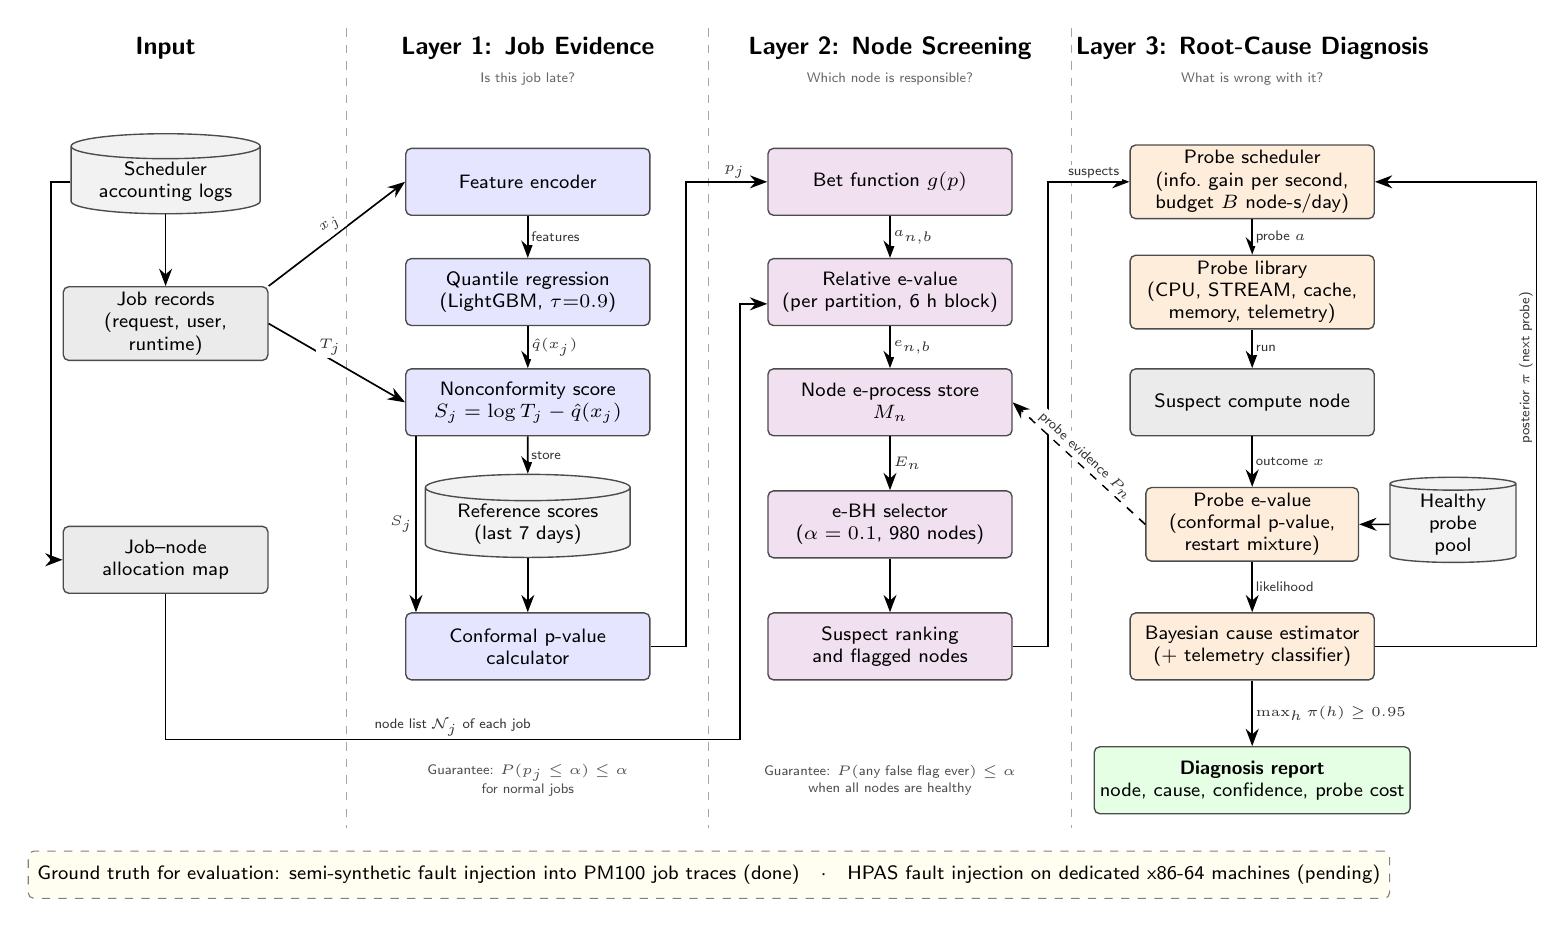
\begin{tikzpicture}[
  font=\sffamily\scriptsize,
  >={Stealth[length=2.2mm]},
  blk/.style={draw=black!70, rounded corners=2pt, align=center, minimum width=31mm,
              minimum height=8.5mm, inner sep=2pt, line width=0.5pt},
  l1/.style={blk, fill=blue!10},
  l2/.style={blk, fill=violet!12},
  l3/.style={blk, fill=orange!14},
  io/.style={blk, fill=black!8},
  store/.style={draw=black!70, cylinder, shape border rotate=90, aspect=0.18, align=center,
                minimum width=24mm, minimum height=10mm, fill=black!5, inner sep=1pt, line width=0.5pt},
  flow/.style={->, line width=0.6pt},
  lab/.style={font=\sffamily\tiny, inner sep=1pt, fill=white, text=black!80},
  head/.style={font=\sffamily\bfseries\small},
  sub/.style={font=\sffamily\tiny, text=black!60}
]
% ---------- column x positions ----------
\def\xA{0}\def\xB{4.6}\def\xC{9.2}\def\xD{13.8}

% ---------- headings ----------
\node[head] at (\xA,0.9) {Input};
\node[head] at (\xB,0.9) {Layer 1: Job Evidence};
\node[sub]  at (\xB,0.5) {Is this job late?};
\node[head] at (\xC,0.9) {Layer 2: Node Screening};
\node[sub]  at (\xC,0.5) {Which node is responsible?};
\node[head] at (\xD,0.9) {Layer 3: Root-Cause Diagnosis};
\node[sub]  at (\xD,0.5) {What is wrong with it?};

% ---------- separators ----------
\foreach \x in {2.3,6.9,11.5} \draw[black!35, dashed] (\x,1.15) -- (\x,-9.0);

% ---------- input ----------
\node[store] (logs) at (\xA,-0.8) {Scheduler\\accounting logs};
\node[io, minimum width=26mm] (feat0) at (\xA,-2.6) {Job records\\(request, user,\\runtime)};
\node[io, minimum width=26mm] (alloc) at (\xA,-5.6) {Job--node\\allocation map};
\draw[flow] (logs) -- (feat0);
\draw[flow] (logs.west) -- ++(-0.25,0) |- (alloc.west);

% ---------- layer 1 ----------
\node[l1] (enc)  at (\xB,-0.8) {Feature encoder};
\node[l1] (qm)   at (\xB,-2.2) {Quantile regression\\(LightGBM, $\tau{=}0.9$)};
\node[l1] (sc)   at (\xB,-3.6) {Nonconformity score\\$S_j=\log T_j-\hat q(x_j)$};
\node[store, minimum width=26mm] (ref) at (\xB,-5.15) {Reference scores\\(last 7 days)};
\node[l1] (cp)   at (\xB,-6.7) {Conformal p-value\\calculator};
\draw[flow] (feat0.north east) -- node[lab, above, sloped]{$x_j$} (enc.west);
\draw[flow] (enc) -- node[lab, right]{features} (qm);
\draw[flow] (qm) -- node[lab, right]{$\hat q(x_j)$} (sc);
\draw[flow] (feat0.east) -- node[lab, above, pos=0.45]{$T_j$} (sc.west);
\draw[flow] ($(sc.south)+(-1.42,0)$) -- node[lab, left]{$S_j$} ($(cp.north)+(-1.42,0)$);
\draw[flow] (sc) -- node[lab, right]{store} (ref);
\draw[flow] (ref) -- (cp);

% ---------- layer 2 ----------
\node[l2] (bet)  at (\xC,-0.8) {Bet function $g(p)$};
\node[l2] (rel)  at (\xC,-2.2) {Relative e-value\\(per partition, 6 h block)};
\node[l2] (ep)   at (\xC,-3.6) {Node e-process store\\$M_n$};
\node[l2] (ebh)  at (\xC,-5.15) {e-BH selector\\($\alpha=0.1$, 980 nodes)};
\node[l2] (rank) at (\xC,-6.7) {Suspect ranking\\and flagged nodes};
\draw[flow] (cp.east) -- ++(0.45,0) |- node[lab, above, pos=0.8]{$p_j$} (bet.west);
\draw[flow] (alloc.south) -- ++(0,-1.85) -| node[lab, above, pos=0.25]{node list $\mathcal N_j$ of each job} ($(rel.west)+(-0.35,-0.15)$) -- ($(rel.west)+(0,-0.15)$);
\draw[flow] (bet) -- node[lab, right]{$a_{n,b}$} (rel);
\draw[flow] (rel) -- node[lab, right]{$e_{n,b}$} (ep);
\draw[flow] (ep) -- node[lab, right]{$E_n$} (ebh);
\draw[flow] (ebh) -- (rank);

% ---------- layer 3 ----------
\node[l3] (sched) at (\xD,-0.8) {Probe scheduler\\(info.\ gain per second,\\budget $B$ node-s/day)};
\node[l3] (lib)   at (\xD,-2.2) {Probe library\\(CPU, STREAM, cache,\\memory, telemetry)};
\node[io, minimum width=31mm] (node) at (\xD,-3.6) {Suspect compute node};
\node[l3, minimum width=27mm] (pe)    at (\xD,-5.15) {Probe e-value\\(conformal p-value,\\restart mixture)};
\node[store, minimum width=16mm] (pool) at (\xD+2.55,-5.15) {Healthy\\probe\\pool};
\node[l3] (bayes) at (\xD,-6.7) {Bayesian cause estimator\\(+ telemetry classifier)};
\draw[flow] (rank.east) -- ++(0.45,0) |- node[lab, above, pos=0.78]{suspects} (sched.west);
\draw[flow] (sched) -- node[lab, right]{probe $a$} (lib);
\draw[flow] (lib) -- node[lab, right]{run} (node);
\draw[flow] (node) -- node[lab, right]{outcome $x$} (pe);
\draw[flow] (pool) -- (pe);
\draw[flow] (pe) -- node[lab, right]{likelihood} (bayes);
\draw[flow] (bayes.east) -- ++(2.05,0) |- node[lab, sloped, above, pos=0.3]{posterior $\pi$ (next probe)} (sched.east);
% feedback of probe evidence to layer 2
\draw[flow, dashed] (pe.west) -- node[lab, sloped, above, pos=0.5]{probe evidence $P_n$} (ep.east);

% ---------- output ----------
\node[io, minimum width=40mm, fill=green!10] (out) at (\xD,-8.4) {\textbf{Diagnosis report}\\node, cause, confidence, probe cost};
\draw[flow] (bayes) -- node[lab, right]{$\max_h \pi(h)\ge 0.95$} (bayes |- out.north);

% ---------- guarantees strip ----------
\node[font=\sffamily\tiny, text=black!70, align=center] at (\xB,-8.4) {Guarantee: $P(p_j\le\alpha)\le\alpha$\\for normal jobs};
\node[font=\sffamily\tiny, text=black!70, align=center] at (\xC,-8.4) {Guarantee: $P(\text{any false flag ever})\le\alpha$\\when all nodes are healthy};

% ---------- evaluation ----------
\node[draw=black!50, dashed, rounded corners=2pt, fill=yellow!6, minimum width=172mm, minimum height=6mm,
      align=center, font=\sffamily\scriptsize] (ev) at (6.9,-9.6)
  {Ground truth for evaluation: semi-synthetic fault injection into PM100 job traces (done)\quad$\cdot$\quad HPAS fault injection on dedicated x86-64 machines (pending)};
\end{tikzpicture}
 inside a figure environment,
% or compile architecture_standalone.tex for a PDF/PNG.
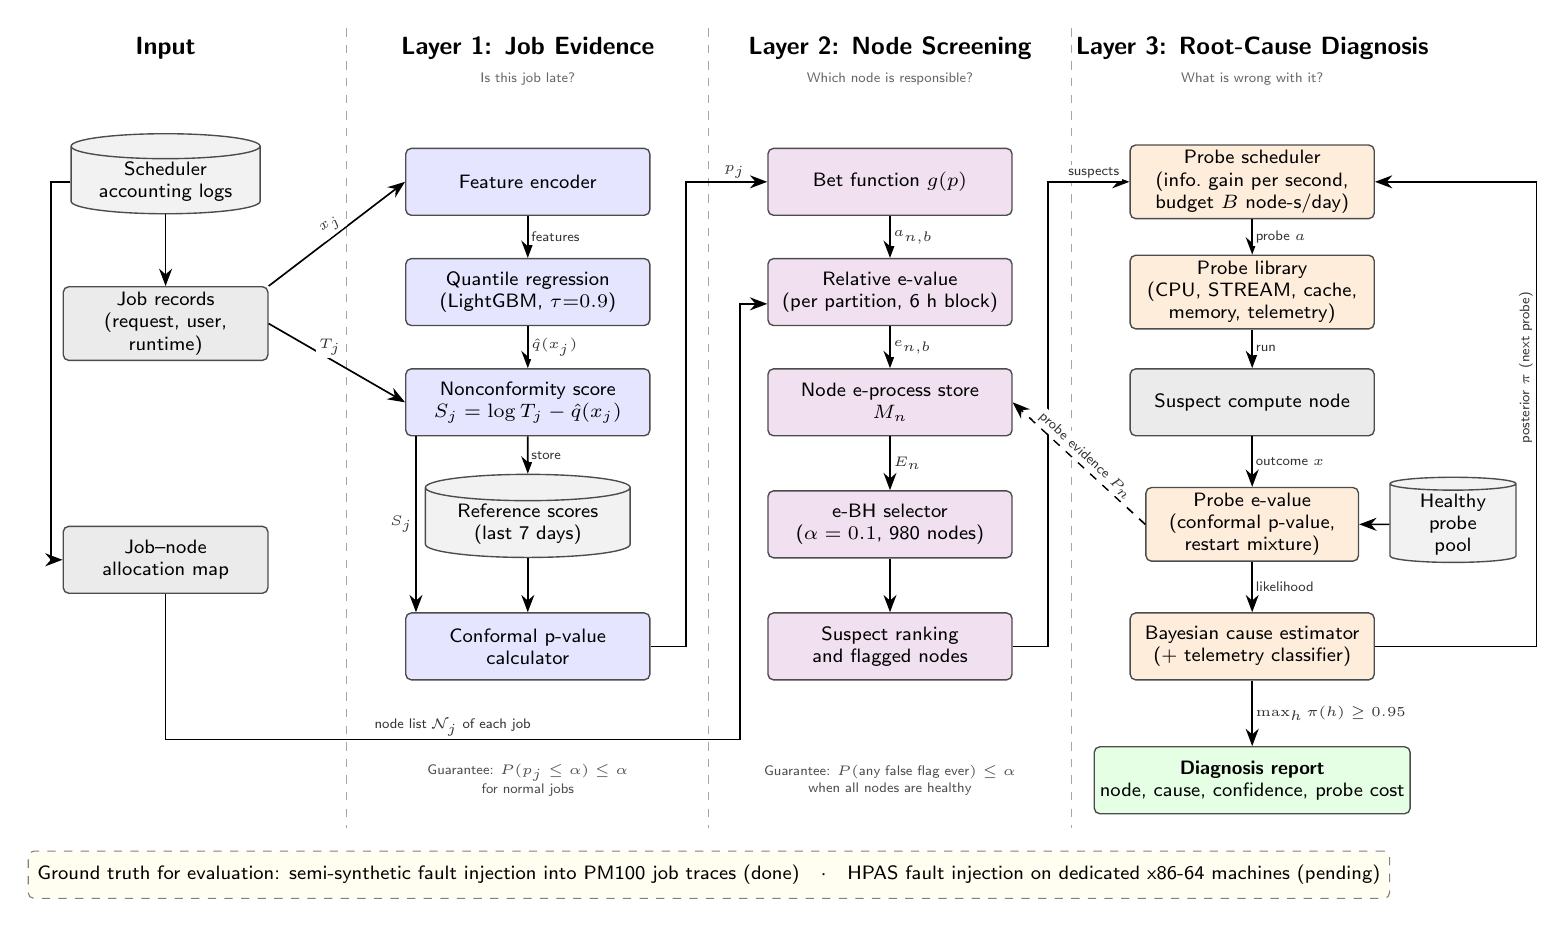
\begin{tikzpicture}[
  font=\sffamily\scriptsize,
  >={Stealth[length=2.2mm]},
  blk/.style={draw=black!70, rounded corners=2pt, align=center, minimum width=31mm,
              minimum height=8.5mm, inner sep=2pt, line width=0.5pt},
  l1/.style={blk, fill=blue!10},
  l2/.style={blk, fill=violet!12},
  l3/.style={blk, fill=orange!14},
  io/.style={blk, fill=black!8},
  store/.style={draw=black!70, cylinder, shape border rotate=90, aspect=0.18, align=center,
                minimum width=24mm, minimum height=10mm, fill=black!5, inner sep=1pt, line width=0.5pt},
  flow/.style={->, line width=0.6pt},
  lab/.style={font=\sffamily\tiny, inner sep=1pt, fill=white, text=black!80},
  head/.style={font=\sffamily\bfseries\small},
  sub/.style={font=\sffamily\tiny, text=black!60}
]
% ---------- column x positions ----------
\def\xA{0}\def\xB{4.6}\def\xC{9.2}\def\xD{13.8}

% ---------- headings ----------
\node[head] at (\xA,0.9) {Input};
\node[head] at (\xB,0.9) {Layer 1: Job Evidence};
\node[sub]  at (\xB,0.5) {Is this job late?};
\node[head] at (\xC,0.9) {Layer 2: Node Screening};
\node[sub]  at (\xC,0.5) {Which node is responsible?};
\node[head] at (\xD,0.9) {Layer 3: Root-Cause Diagnosis};
\node[sub]  at (\xD,0.5) {What is wrong with it?};

% ---------- separators ----------
\foreach \x in {2.3,6.9,11.5} \draw[black!35, dashed] (\x,1.15) -- (\x,-9.0);

% ---------- input ----------
\node[store] (logs) at (\xA,-0.8) {Scheduler\\accounting logs};
\node[io, minimum width=26mm] (feat0) at (\xA,-2.6) {Job records\\(request, user,\\runtime)};
\node[io, minimum width=26mm] (alloc) at (\xA,-5.6) {Job--node\\allocation map};
\draw[flow] (logs) -- (feat0);
\draw[flow] (logs.west) -- ++(-0.25,0) |- (alloc.west);

% ---------- layer 1 ----------
\node[l1] (enc)  at (\xB,-0.8) {Feature encoder};
\node[l1] (qm)   at (\xB,-2.2) {Quantile regression\\(LightGBM, $\tau{=}0.9$)};
\node[l1] (sc)   at (\xB,-3.6) {Nonconformity score\\$S_j=\log T_j-\hat q(x_j)$};
\node[store, minimum width=26mm] (ref) at (\xB,-5.15) {Reference scores\\(last 7 days)};
\node[l1] (cp)   at (\xB,-6.7) {Conformal p-value\\calculator};
\draw[flow] (feat0.north east) -- node[lab, above, sloped]{$x_j$} (enc.west);
\draw[flow] (enc) -- node[lab, right]{features} (qm);
\draw[flow] (qm) -- node[lab, right]{$\hat q(x_j)$} (sc);
\draw[flow] (feat0.east) -- node[lab, above, pos=0.45]{$T_j$} (sc.west);
\draw[flow] ($(sc.south)+(-1.42,0)$) -- node[lab, left]{$S_j$} ($(cp.north)+(-1.42,0)$);
\draw[flow] (sc) -- node[lab, right]{store} (ref);
\draw[flow] (ref) -- (cp);

% ---------- layer 2 ----------
\node[l2] (bet)  at (\xC,-0.8) {Bet function $g(p)$};
\node[l2] (rel)  at (\xC,-2.2) {Relative e-value\\(per partition, 6 h block)};
\node[l2] (ep)   at (\xC,-3.6) {Node e-process store\\$M_n$};
\node[l2] (ebh)  at (\xC,-5.15) {e-BH selector\\($\alpha=0.1$, 980 nodes)};
\node[l2] (rank) at (\xC,-6.7) {Suspect ranking\\and flagged nodes};
\draw[flow] (cp.east) -- ++(0.45,0) |- node[lab, above, pos=0.8]{$p_j$} (bet.west);
\draw[flow] (alloc.south) -- ++(0,-1.85) -| node[lab, above, pos=0.25]{node list $\mathcal N_j$ of each job} ($(rel.west)+(-0.35,-0.15)$) -- ($(rel.west)+(0,-0.15)$);
\draw[flow] (bet) -- node[lab, right]{$a_{n,b}$} (rel);
\draw[flow] (rel) -- node[lab, right]{$e_{n,b}$} (ep);
\draw[flow] (ep) -- node[lab, right]{$E_n$} (ebh);
\draw[flow] (ebh) -- (rank);

% ---------- layer 3 ----------
\node[l3] (sched) at (\xD,-0.8) {Probe scheduler\\(info.\ gain per second,\\budget $B$ node-s/day)};
\node[l3] (lib)   at (\xD,-2.2) {Probe library\\(CPU, STREAM, cache,\\memory, telemetry)};
\node[io, minimum width=31mm] (node) at (\xD,-3.6) {Suspect compute node};
\node[l3, minimum width=27mm] (pe)    at (\xD,-5.15) {Probe e-value\\(conformal p-value,\\restart mixture)};
\node[store, minimum width=16mm] (pool) at (\xD+2.55,-5.15) {Healthy\\probe\\pool};
\node[l3] (bayes) at (\xD,-6.7) {Bayesian cause estimator\\(+ telemetry classifier)};
\draw[flow] (rank.east) -- ++(0.45,0) |- node[lab, above, pos=0.78]{suspects} (sched.west);
\draw[flow] (sched) -- node[lab, right]{probe $a$} (lib);
\draw[flow] (lib) -- node[lab, right]{run} (node);
\draw[flow] (node) -- node[lab, right]{outcome $x$} (pe);
\draw[flow] (pool) -- (pe);
\draw[flow] (pe) -- node[lab, right]{likelihood} (bayes);
\draw[flow] (bayes.east) -- ++(2.05,0) |- node[lab, sloped, above, pos=0.3]{posterior $\pi$ (next probe)} (sched.east);
% feedback of probe evidence to layer 2
\draw[flow, dashed] (pe.west) -- node[lab, sloped, above, pos=0.5]{probe evidence $P_n$} (ep.east);

% ---------- output ----------
\node[io, minimum width=40mm, fill=green!10] (out) at (\xD,-8.4) {\textbf{Diagnosis report}\\node, cause, confidence, probe cost};
\draw[flow] (bayes) -- node[lab, right]{$\max_h \pi(h)\ge 0.95$} (bayes |- out.north);

% ---------- guarantees strip ----------
\node[font=\sffamily\tiny, text=black!70, align=center] at (\xB,-8.4) {Guarantee: $P(p_j\le\alpha)\le\alpha$\\for normal jobs};
\node[font=\sffamily\tiny, text=black!70, align=center] at (\xC,-8.4) {Guarantee: $P(\text{any false flag ever})\le\alpha$\\when all nodes are healthy};

% ---------- evaluation ----------
\node[draw=black!50, dashed, rounded corners=2pt, fill=yellow!6, minimum width=172mm, minimum height=6mm,
      align=center, font=\sffamily\scriptsize] (ev) at (6.9,-9.6)
  {Ground truth for evaluation: semi-synthetic fault injection into PM100 job traces (done)\quad$\cdot$\quad HPAS fault injection on dedicated x86-64 machines (pending)};
\end{tikzpicture}
 inside a figure environment,
% or compile architecture_standalone.tex for a PDF/PNG.
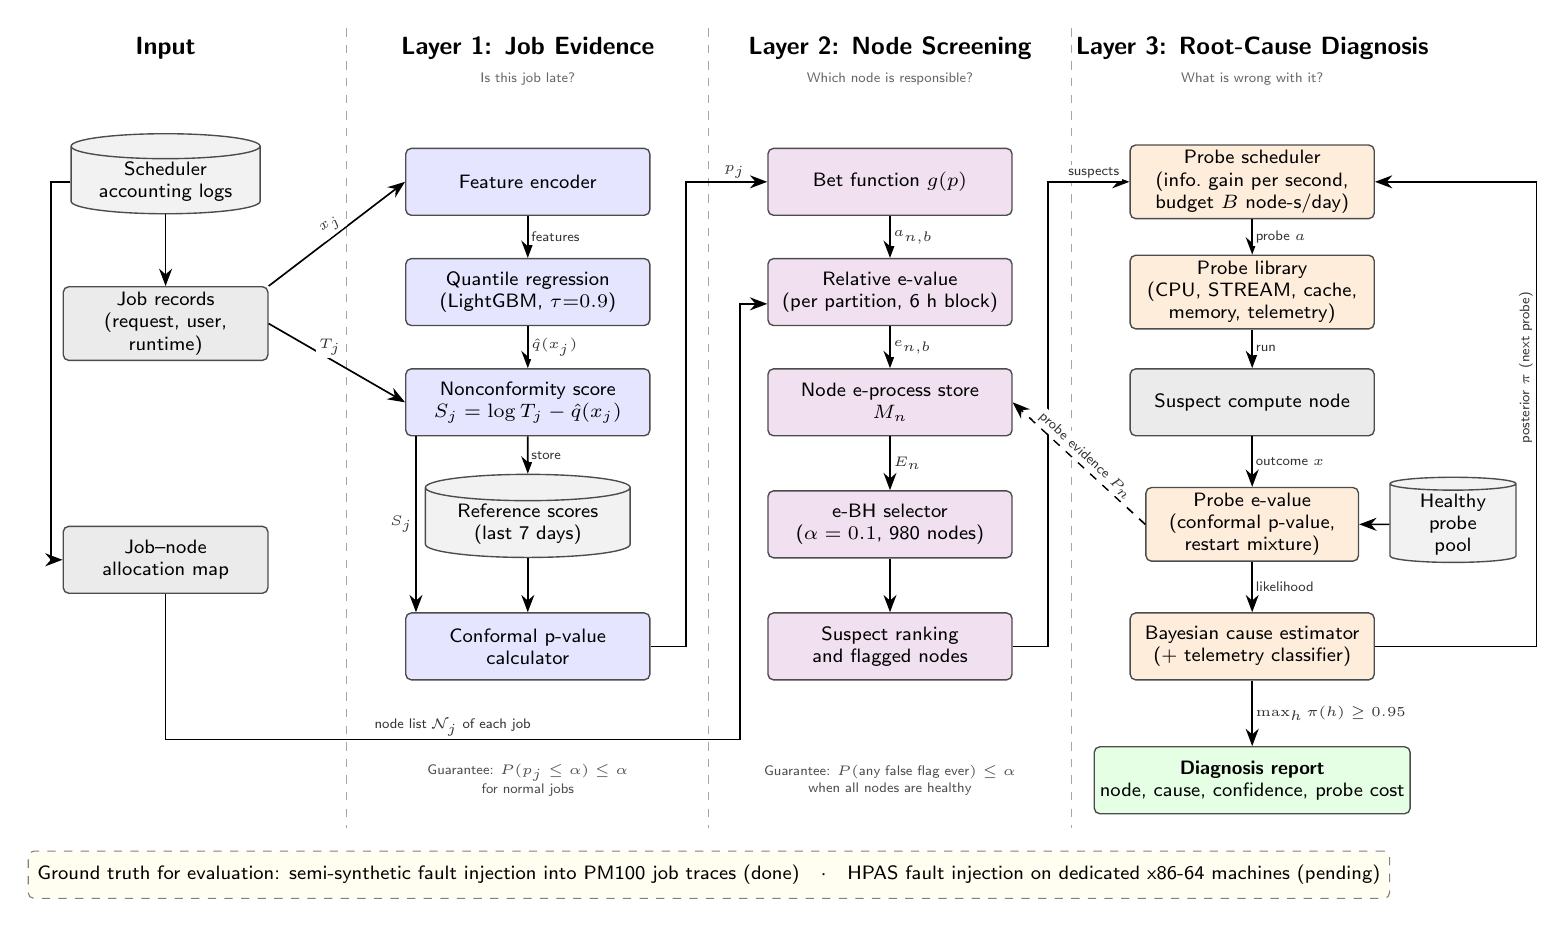
\begin{tikzpicture}[
  font=\sffamily\scriptsize,
  >={Stealth[length=2.2mm]},
  blk/.style={draw=black!70, rounded corners=2pt, align=center, minimum width=31mm,
              minimum height=8.5mm, inner sep=2pt, line width=0.5pt},
  l1/.style={blk, fill=blue!10},
  l2/.style={blk, fill=violet!12},
  l3/.style={blk, fill=orange!14},
  io/.style={blk, fill=black!8},
  store/.style={draw=black!70, cylinder, shape border rotate=90, aspect=0.18, align=center,
                minimum width=24mm, minimum height=10mm, fill=black!5, inner sep=1pt, line width=0.5pt},
  flow/.style={->, line width=0.6pt},
  lab/.style={font=\sffamily\tiny, inner sep=1pt, fill=white, text=black!80},
  head/.style={font=\sffamily\bfseries\small},
  sub/.style={font=\sffamily\tiny, text=black!60}
]
% ---------- column x positions ----------
\def\xA{0}\def\xB{4.6}\def\xC{9.2}\def\xD{13.8}

% ---------- headings ----------
\node[head] at (\xA,0.9) {Input};
\node[head] at (\xB,0.9) {Layer 1: Job Evidence};
\node[sub]  at (\xB,0.5) {Is this job late?};
\node[head] at (\xC,0.9) {Layer 2: Node Screening};
\node[sub]  at (\xC,0.5) {Which node is responsible?};
\node[head] at (\xD,0.9) {Layer 3: Root-Cause Diagnosis};
\node[sub]  at (\xD,0.5) {What is wrong with it?};

% ---------- separators ----------
\foreach \x in {2.3,6.9,11.5} \draw[black!35, dashed] (\x,1.15) -- (\x,-9.0);

% ---------- input ----------
\node[store] (logs) at (\xA,-0.8) {Scheduler\\accounting logs};
\node[io, minimum width=26mm] (feat0) at (\xA,-2.6) {Job records\\(request, user,\\runtime)};
\node[io, minimum width=26mm] (alloc) at (\xA,-5.6) {Job--node\\allocation map};
\draw[flow] (logs) -- (feat0);
\draw[flow] (logs.west) -- ++(-0.25,0) |- (alloc.west);

% ---------- layer 1 ----------
\node[l1] (enc)  at (\xB,-0.8) {Feature encoder};
\node[l1] (qm)   at (\xB,-2.2) {Quantile regression\\(LightGBM, $\tau{=}0.9$)};
\node[l1] (sc)   at (\xB,-3.6) {Nonconformity score\\$S_j=\log T_j-\hat q(x_j)$};
\node[store, minimum width=26mm] (ref) at (\xB,-5.15) {Reference scores\\(last 7 days)};
\node[l1] (cp)   at (\xB,-6.7) {Conformal p-value\\calculator};
\draw[flow] (feat0.north east) -- node[lab, above, sloped]{$x_j$} (enc.west);
\draw[flow] (enc) -- node[lab, right]{features} (qm);
\draw[flow] (qm) -- node[lab, right]{$\hat q(x_j)$} (sc);
\draw[flow] (feat0.east) -- node[lab, above, pos=0.45]{$T_j$} (sc.west);
\draw[flow] ($(sc.south)+(-1.42,0)$) -- node[lab, left]{$S_j$} ($(cp.north)+(-1.42,0)$);
\draw[flow] (sc) -- node[lab, right]{store} (ref);
\draw[flow] (ref) -- (cp);

% ---------- layer 2 ----------
\node[l2] (bet)  at (\xC,-0.8) {Bet function $g(p)$};
\node[l2] (rel)  at (\xC,-2.2) {Relative e-value\\(per partition, 6 h block)};
\node[l2] (ep)   at (\xC,-3.6) {Node e-process store\\$M_n$};
\node[l2] (ebh)  at (\xC,-5.15) {e-BH selector\\($\alpha=0.1$, 980 nodes)};
\node[l2] (rank) at (\xC,-6.7) {Suspect ranking\\and flagged nodes};
\draw[flow] (cp.east) -- ++(0.45,0) |- node[lab, above, pos=0.8]{$p_j$} (bet.west);
\draw[flow] (alloc.south) -- ++(0,-1.85) -| node[lab, above, pos=0.25]{node list $\mathcal N_j$ of each job} ($(rel.west)+(-0.35,-0.15)$) -- ($(rel.west)+(0,-0.15)$);
\draw[flow] (bet) -- node[lab, right]{$a_{n,b}$} (rel);
\draw[flow] (rel) -- node[lab, right]{$e_{n,b}$} (ep);
\draw[flow] (ep) -- node[lab, right]{$E_n$} (ebh);
\draw[flow] (ebh) -- (rank);

% ---------- layer 3 ----------
\node[l3] (sched) at (\xD,-0.8) {Probe scheduler\\(info.\ gain per second,\\budget $B$ node-s/day)};
\node[l3] (lib)   at (\xD,-2.2) {Probe library\\(CPU, STREAM, cache,\\memory, telemetry)};
\node[io, minimum width=31mm] (node) at (\xD,-3.6) {Suspect compute node};
\node[l3, minimum width=27mm] (pe)    at (\xD,-5.15) {Probe e-value\\(conformal p-value,\\restart mixture)};
\node[store, minimum width=16mm] (pool) at (\xD+2.55,-5.15) {Healthy\\probe\\pool};
\node[l3] (bayes) at (\xD,-6.7) {Bayesian cause estimator\\(+ telemetry classifier)};
\draw[flow] (rank.east) -- ++(0.45,0) |- node[lab, above, pos=0.78]{suspects} (sched.west);
\draw[flow] (sched) -- node[lab, right]{probe $a$} (lib);
\draw[flow] (lib) -- node[lab, right]{run} (node);
\draw[flow] (node) -- node[lab, right]{outcome $x$} (pe);
\draw[flow] (pool) -- (pe);
\draw[flow] (pe) -- node[lab, right]{likelihood} (bayes);
\draw[flow] (bayes.east) -- ++(2.05,0) |- node[lab, sloped, above, pos=0.3]{posterior $\pi$ (next probe)} (sched.east);
% feedback of probe evidence to layer 2
\draw[flow, dashed] (pe.west) -- node[lab, sloped, above, pos=0.5]{probe evidence $P_n$} (ep.east);

% ---------- output ----------
\node[io, minimum width=40mm, fill=green!10] (out) at (\xD,-8.4) {\textbf{Diagnosis report}\\node, cause, confidence, probe cost};
\draw[flow] (bayes) -- node[lab, right]{$\max_h \pi(h)\ge 0.95$} (bayes |- out.north);

% ---------- guarantees strip ----------
\node[font=\sffamily\tiny, text=black!70, align=center] at (\xB,-8.4) {Guarantee: $P(p_j\le\alpha)\le\alpha$\\for normal jobs};
\node[font=\sffamily\tiny, text=black!70, align=center] at (\xC,-8.4) {Guarantee: $P(\text{any false flag ever})\le\alpha$\\when all nodes are healthy};

% ---------- evaluation ----------
\node[draw=black!50, dashed, rounded corners=2pt, fill=yellow!6, minimum width=172mm, minimum height=6mm,
      align=center, font=\sffamily\scriptsize] (ev) at (6.9,-9.6)
  {Ground truth for evaluation: semi-synthetic fault injection into PM100 job traces (done)\quad$\cdot$\quad HPAS fault injection on dedicated x86-64 machines (pending)};
\end{tikzpicture}
}
\caption{System architecture. Layer~1 converts each finished job into a conformal p-value; Layer~2 turns p-values into per-node evidence and selects nodes with e-BH; Layer~3 probes the highest-ranked suspects within a daily budget, feeds probe evidence back to Layer~2 and reports the cause.}
\label{fig:arch}
\end{figure}

\subsection{Layer 1: Conformal job evidence}
A gradient-boosted quantile model (LightGBM~\cite{lightgbm}, $\tau = 0.9$, 200 trees, learning rate 0.05, 50 leaves) predicts the 0.9-quantile $\hat q(x_j)$ of log runtime from submission features $x_j$: requested walltime, cores, memory, nodes and GPUs (numeric), user and partition (categorical). It is trained on the first 45 days of the trace (window chosen by pinball loss among 30, 45 and 60 days) and then frozen on 19 June 2020. The nonconformity score of job $j$ with runtime $T_j$ is
\begin{equation}
S_j = \log T_j - \hat q(x_j).
\end{equation}
A larger $S_j$ means the job took longer than predicted. The reference set $R_j$ holds the scores of all jobs that ended in the 7 days before job $j$ (at least 30 jobs). With a uniform random tie-breaker $\theta_j$,
\begin{equation}
p_j = \frac{\#\{i \in R_j : S_i > S_j\} + \theta_j\,\bigl(1 + \#\{i \in R_j : S_i = S_j\}\bigr)}{|R_j| + 1}.
\end{equation}
\textbf{Interpretation.} $p_j$ is the fraction of recent comparable jobs that were even later, relative to their prediction, than job $j$. A small $p_j$ (for example 0.001) means that almost no recent job was this late, so the job is in the extreme slow tail. If job $j$ is exchangeable with the jobs in $R_j$, then $P(p_j \le \alpha) = \alpha$ exactly~\cite{cqr}: a threshold of 0.05 raises an alarm on 5\% of normal jobs, whatever the runtime distribution. The prediction model does not need to be accurate for this guarantee; a better model only makes slow jobs stand out more.

\subsection{Layer 2: Node screening with relative e-values}
Time is cut into 6-hour blocks $b$. Every job that ends in block $b$ contributes a bet $g(p_j)$ to each node in its node list $\mathcal N_j$, where $g$ is a histogram likelihood ratio, built on a warm-up week, between the p-value distribution of jobs slowed by a factor $s_0$ and the uniform distribution. Let $a_{n,b}$ be the mean bet of node $n$'s jobs in the block and $A_{q,b}$ the nodes of partition $q$ that ran a job in the block. The relative e-value is
\begin{equation}
e_{n,b} = \frac{a_{n,b}}{\frac{1}{|A_{q,b}|}\sum_{m \in A_{q,b}} a_{m,b}}.
\end{equation}
\textbf{Property.} If jobs are placed on nodes without regard to node identity (random placement within a partition), then $\mathbb E[e_{n,b} \mid \text{past}] = 1$ exactly for any mix of job sizes and any dependence between jobs, because the ratios always sum to $|A_{q,b}|$ and the node labels are exchangeable. A system-wide slowdown raises numerator and denominator together and creates no evidence.

The node evidence $M_n$ multiplies $e_{n,b}$ over time inside a mixture over a ``no fault yet'' state and bets for $s_0 \in \{1.2, 1.3, 1.5, 2.0, 3.0\}$, with switching rate $J = 0.01$, so that a fault can start at any time without the evidence collected before it working against detection. Every 6 hours the e-BH procedure~\cite{ebh} at level $\alpha = 0.1$ over all $m = 980$ nodes flags the $k^\ast$ nodes with the largest evidence, where $k^\ast$ is the largest $k$ such that the $k$-th largest evidence is at least $m/(\alpha k)$.

\textbf{Guarantee.} When all nodes are healthy, a flag requires the average evidence over the 980 nodes to reach $1/\alpha$. That average is a non-negative supermartingale starting at 1, so by Ville's inequality the probability that any node is ever flagged is at most $\alpha$, at any time the operator looks.

\subsection{Layer 3: Cost-aware active probing and diagnosis}
\textbf{Probes.} Four micro-benchmarks and one telemetry capture, each run on a single node: CPU fixed-work timing (20\,s), STREAM memory bandwidth (20\,s), cache pointer chase (20\,s), free memory (1\,s), and a telemetry snapshot (60\,s). The design model for probe $a$ on a node with cause $h$ and slowdown $s$ is $\log x \sim \mathcal N(k_{h,a} \log s, \sigma^2)$ with $\sigma = 0.05$; Phase~6 replaces these assumed values with measurements.

\textbf{Probe evidence.} Each probe outcome is compared with a pool of 1{,}000 healthy runs of the same probe (a conformal p-value) and converted into an e-value $f_a$ by a bet over the current posterior on (cause, slowdown). A node is probed in investigations $i = 1, 2, \dots$ with factors $F_i$; their evidence is combined by a \emph{restart mixture}
\begin{equation}
P_n = \sum_{k \le N} J(1-J)^{k-1}\prod_{i=k}^{N} F_i + (1-J)^N, \qquad E_n = M_n \cdot P_n,
\end{equation}
which keeps the Layer~2 guarantee while limiting the cost of probes run before a fault starts to about $\log(1/J) = 4.6$ nats.

\textbf{Probe selection and diagnosis.} A budget of $B$ node-seconds per day is released every 6 hours. Nodes are investigated in decreasing order of $E_n$. The next probe maximises the expected information gain about (cause, slowdown) per second of probe cost~\cite{rish}:
\begin{equation}
a^\ast = \arg\max_a \frac{H(\pi) - \mathbb E_{o}\bigl[H(\pi \mid o, a)\bigr]}{c_a}.
\end{equation}
The posterior over causes $\{$healthy, CPU, cache, memory bandwidth, memory leak$\}$ $\times$ slowdown is updated by Bayes' rule; the telemetry probe's likelihood is the confusion matrix of a random-forest classifier trained on the Antarex fault dataset~\cite{antarex}. A node whose cause posterior reaches 0.95 is reported with its cause; a node whose healthy posterior reaches 0.95 is cleared for 7 days.

% ------------------------------------------------------------------ 7
\section{Datasets and Experimental Setup}
\begin{table}[H]
\centering
\caption{Datasets (all public).}
\label{tab:data}
\small
\begin{tabularx}{\textwidth}{@{}lXl@{}}
\toprule
Dataset & Content and use & Source \\
\midrule
PM100~\cite{pm100} & Marconi100 (CINECA): 231{,}238 jobs, 980 nodes in 3 partitions, May--Oct 2020, with the node list of each job. Main dataset for Layers 1--3 & Zenodo 10127767, CC-BY 4.0\\
NREL Eagle~\cite{eagle} & 11 million jobs, no node lists. Layer~1 baseline (reproduction of~\cite{menear}) and second calibration check & OEDI submission 5860\\
Antarex~\cite{antarex} & Node telemetry with injected CPU, cache, memory-bandwidth and memory-leak faults. Telemetry probe classifier & doi:10.5281/zenodo.2553224\\
Prodigy~\cite{prodigy} & Eclipse telemetry: healthy, CPU occupation, memory leak. Classifier check (mid-review prototype and multi-class check) & doi:10.5281/zenodo.8079388\\
\bottomrule
\end{tabularx}
\end{table}

\textbf{Ground truth by injection.} Real job placements carry no fault labels. We therefore re-place jobs at random within their partition and multiply the runtime of every job that touches a chosen set of nodes by a slowdown $s \in \{1.1, 1.2, 1.3, 1.5, 2.0, 3.0\}$, from a random onset date. $K \in \{1, 2, 5\}\%$ of nodes are degraded. \emph{Null} scenarios inject nothing; \emph{decoy} scenarios slow a user, a heavy user, or the whole system instead of a node, and must not raise flags. 3{,}281 scenarios were generated.

\textbf{Metrics.} \emph{Validity}: probability that any node is ever flagged in a null or decoy scenario, $P(\text{ever})$, required to be at most $\alpha + 2$ standard errors. \emph{Speed}: Kaplan--Meier probability that a degraded node is flagged within 14 days of onset, $F(14\,\mathrm{d})$, and recall by the end of the trace. \emph{Diagnosis}: share of flagged degraded nodes whose reported cause is correct. \emph{Cost}: node-seconds of probing per day.

\textbf{Discipline.} Development used scenario seeds 0--19 and 200 null placements. Seeds 20--39 and a further 200 null placements are sealed: they are run once, after the method is frozen, with pass marks fixed in advance (validity at every budget; $F(14\,\mathrm{d}) \ge 0.8$ and accuracy $\ge 0.9$ at $B = 7{,}200$). All results in this report are development results.

% ------------------------------------------------------------------ 8
\section{Implementation}
The system is written in Python (pandas, DuckDB, LightGBM, scikit-learn, NumPy) as one package with a module per layer, YAML configuration files and a run registry that records the configuration hash, git commit and key metrics of every run. Each phase ended with a written report and a pre-registered pass/fail gate.

\begin{table}[H]
\centering
\caption{Development phases and gates.}
\label{tab:phases}
\small
\begin{tabularx}{\textwidth}{@{}lXl@{}}
\toprule
Phase & Work & Gate result \\
\midrule
0 & Data download with checksums, cleaning, profiling of PM100 and Eagle & Pass\\
1 & Layer~1 baseline: reproduce Menear et al.~\cite{menear} on Eagle & Pass (RMSE 7.38\,h vs 8.14\,h reported)\\
2 & Layer~1: quantile model, conformal p-values, adaptive conformal inference & Pass on PM100 main set\\
3 & Fault-injection scenarios with exact ground truth & Pass\\
4, 4b, 4c & Layer~2: node e-processes, e-BH, burst-robust relative e-values & Validity pass; logs-only speed \textbf{fail}\\
5, 5b, 5c & Layer~3: probes, information-gain scheduler, Bayesian diagnosis, restart mixture & Validity and diagnosis pass; small-budget speed \textbf{fail}\\
6-prep & Real-hardware measurement kit (HPAS harness, safety interlocks, analysis) & Built and tested; not yet run\\
\bottomrule
\end{tabularx}
\end{table}

\textbf{Quality controls.} 460 automated tests (unit tests of every formula against brute-force computations, exactness tests of the e-values, safety interlocks of the measurement kit). The method was frozen as git tag \texttt{v1.0-dev-frozen}; a guard script refuses to run the sealed evaluation if any method file differs from the frozen version. Every failed check and design error is recorded in the decision log (120 decisions to date).

% ------------------------------------------------------------------ 9
\section{Results}
All results below are on development data. Layer~3 results use the assumed probe model.

\subsection{Layer 1: runtime model and p-values}
Table~\ref{tab:l1pred} evaluates the frozen model on the 102{,}120 PM100 jobs that ended after the freeze date. The median model predicts runtime roughly twice as well as simple baselines, but runtime prediction from submission data remains hard: only 37.2\% of predictions are within a factor of two. This does not affect the false-alarm guarantee, which comes from the conformal step (Table~\ref{tab:l1cal}).

\begin{table}[H]
\centering
\caption{Layer~1 prediction accuracy, PM100, 102{,}120 jobs after the freeze (median model unless stated).}
\label{tab:l1pred}
\small
\begin{tabular}{@{}lccc@{}}
\toprule
Metric & LightGBM (ours) & Constant median & Requested walltime\\
\midrule
Predictions within $2\times$ of actual runtime & \textbf{37.2\%} & 19.5\% & 18.6\%\\
RMSE (hours) & \textbf{5.55} & 6.24 & 11.28\\
MAE (hours) & 2.78 & 2.55 & 7.18\\
$R^2$ on log runtime & \textbf{0.06} & 0.00 & $-1.07$\\
Spearman rank correlation & 0.49 & -- & --\\
Coverage of the 0.9-quantile (target 0.90) & 0.874 & -- & --\\
Pinball loss of the 0.9-quantile (log runtime) & 0.243 & -- & --\\
\bottomrule
\end{tabular}
\end{table}

On Eagle, our Phase~1 reproduction of Menear et al.\ reached a pooled RMSE of 7.38\,h over 1{,}358{,}770 test jobs, against 8.14\,h reported in~\cite{menear}.

\begin{table}[H]
\centering
\caption{Layer~1 p-value calibration, PM100 (frozen model). Under perfect calibration the share of jobs with $p \le \alpha$ equals $\alpha$ and the KS distance is 0.}
\label{tab:l1cal}
\small
\begin{tabular}{@{}lccccc@{}}
\toprule
Reference set & Jobs & KS & $p \le 0.01$ & $p \le 0.05$ & $p \le 0.10$\\
\midrule
Per user (mid-review plan) & 102{,}120 & 0.091 & 0.023 & 0.086 & 0.155\\
Pooled, previous 7 days (final) & 102{,}090 & \textbf{0.013} & \textbf{0.0125} & \textbf{0.0523} & \textbf{0.0997}\\
\bottomrule
\end{tabular}
\end{table}

The extreme tail is also calibrated: 0.124\% of jobs have $p \le 0.001$ (limit 0.2\%). On the later part of the trace alone (test days from day 90), the KS distance is 0.023, slightly above the 0.02 target, while the alarm rates stay within $\pm 0.01$ of $\alpha$.

\subsection{Layer 2: node screening from scheduler logs alone}
Table~\ref{tab:l2base} compares Layer~2 with node-flagging rules from practice and the literature on the same scenarios. Every threshold or ranking rule flags at least one healthy node in every null scenario; the e-value methods stay below $\alpha = 0.1$.

\begin{table}[H]
\centering
\caption{Layer~2 against baselines (Phase~4; null and decoy: $P(\text{ever})$, $\alpha = 0.1$; detection at $K = 1\%$, $s = 1.3$).}
\label{tab:l2base}
\small
\begin{tabularx}{\textwidth}{@{}Xcccc@{}}
\toprule
Method & Null $P$(ever) & Decoy $P$(ever) & Recall by end & False discovery prop.\\
\midrule
Threshold rule (median residual $>20\%$, $\ge 10$ jobs, $\ge 3$ users) & 1.000 & 1.000 & 0.873 & 0.484\\
Top 5\% of nodes by residual & 1.000 & 1.000 & 0.527 & 0.994\\
Fisher combination + BH & 1.000 & 1.000 & 0.680 & 0.538\\
Ours, e-processes (Phase~4 version) & \textbf{0.040} & \textbf{0.050} & 0.807 & \textbf{0.013}\\
\bottomrule
\end{tabularx}
\end{table}

\textbf{Bursts of slow jobs.} On the real job stream, slow jobs arrive in bursts (the lag-1 autocorrelation of $\mathbf 1\{p < 0.1\}$ is 0.29). The weighted e-value of the mid-review design then flagged a healthy node in 98.5\% of null scenarios; the relative e-value reduced this to 7.0\% (200 null scenarios) and was adopted. Decoy and system-shock scenarios were never flagged.

\begin{table}[H]
\centering
\caption{Layer~2 alone (no probes, $B = 0$), $K = 1\%$: share of degraded nodes flagged.}
\label{tab:l2speed}
\small
\begin{tabular}{@{}lcccccc@{}}
\toprule
Slowdown $s$ & 1.1 & 1.2 & 1.3 & 1.5 & 2.0 & 3.0\\
\midrule
Within 14 days, $F(14\,\mathrm{d})$ & 0.040 & 0.085 & 0.115 & 0.115 & 0.175 & 0.200\\
By end of trace & 0.335 & 0.585 & 0.725 & 0.825 & 0.870 & 0.870\\
\bottomrule
\end{tabular}
\end{table}

Logs alone eventually find most degraded nodes but slowly: the 14-day target of 0.8 (Gate~4b) is not met. A single degraded node among 980 changes few job runtimes, and each job is weak evidence. This is the motivation for Layer~3.

\subsection{Layer 3: probing and diagnosis}\label{sec:l3res}
\begin{table}[H]
\centering
\caption{Full system against probing budget, $K = 1\%$, $s = 1.3$, $\alpha = 0.1$ (200 null scenarios; 20 seeds).}
\label{tab:l3budget}
\small
\begin{tabular}{@{}rcccccc@{}}
\toprule
$B$ (node-s/day) & Cluster time & Null $P$(ever) & $F(14\,\mathrm{d})$ & Recall by end & Accuracy & s/investigation\\
\midrule
0 & 0 & 0.070 & 0.115 & 0.725 & -- & --\\
300 & 0.0004\% & 0.065 & 0.505 & 0.945 & 0.990 & 41.1\\
1{,}800 & 0.002\% & 0.065 & 0.830 & 0.995 & 0.991 & 64.9\\
7{,}200 & 0.0085\% & 0.065 & \textbf{0.985} & \textbf{1.000} & \textbf{0.991} & 71.0\\
\bottomrule
\end{tabular}
\end{table}

\begin{table}[H]
\centering
\caption{$F(14\,\mathrm{d})$ by slowdown and share of degraded nodes, $B = 7{,}200$ node-s/day.}
\label{tab:l3grid}
\small
\begin{tabular}{@{}lcccccc@{}}
\toprule
$K$ & $s=1.1$ & 1.2 & 1.3 & 1.5 & 2.0 & 3.0\\
\midrule
1\% & 0.155 & 0.975 & 0.985 & 0.985 & 0.995 & 1.000\\
2\% & 0.180 & 0.965 & 0.980 & 0.995 & 0.995 & 0.992\\
5\% & 0.179 & 0.943 & 0.977 & 0.988 & 0.994 & 0.995\\
\bottomrule
\end{tabular}
\end{table}

\textbf{Value of Layer~2 ranking.} With the same budget ($B = 1{,}800$, first Layer~3 version), probing the nodes ranked by Layer~2 flagged 60.0\% of degraded nodes within 14 days, against 13.5\% when probing random nodes and 12.0\% when sweeping all nodes in turn.

\textbf{Probe debt and the restart mixture.} In the first Layer~3 design, every probe result was multiplied into the node evidence permanently. Each probe of a still-healthy node then cost about 2.1 nats of evidence that was never recovered. Table~\ref{tab:debt} adds healthy investigations before the fault begins, as happens in a long deployment.

\begin{table}[H]
\centering
\caption{Effect of earlier healthy investigations on $F(14\,\mathrm{d})$, $K = 1\%$, $s = 1.3$, $B = 7{,}200$.}
\label{tab:debt}
\small
\begin{tabular}{@{}lccc@{}}
\toprule
Extra healthy investigations before onset & 0 & 10 ($\approx$2 months) & 25 ($\approx$5 months)\\
\midrule
Product of probe factors (first design) & 0.965 & 0.245 & 0.000\\
Restart mixture (final) & \textbf{0.985} & \textbf{0.975} & \textbf{0.930}\\
\bottomrule
\end{tabular}
\end{table}

\textbf{Sensitivity to the probe model.} If the true probe responses differ from the assumed ones by $\pm 50\%$ and the noise is doubled, validity still holds ($P(\text{ever}) \le 0.065$), but $F(14\,\mathrm{d})$ at $B = 7{,}200$ falls from 0.985 to 0.615 and cause accuracy from 0.991 to 0.889. Measuring the real probe behaviour (Phase~6) is therefore the most important remaining step.

\subsection{Telemetry classifier (Layer 3 telemetry probe)}
\begin{table}[H]
\centering
\caption{Random-forest telemetry classifier.}
\label{tab:tel}
\small
\begin{tabularx}{\textwidth}{@{}Xll@{}}
\toprule
Setting & Classes & Macro-F1\\
\midrule
Prodigy, grouped 5-fold CV (mid-review prototype) & healthy, anomalous & 0.970\\
Prodigy, grouped by job & healthy, CPU occupation, memory leak & 0.883\\
Antarex, contiguous time folds, same configuration & healthy, CPU, cache, memory bandwidth, memory leak & 1.000\\
Antarex, train on one configuration, test on the other & same five classes & 0.69 / 0.85\\
\bottomrule
\end{tabularx}
\end{table}

The perfect within-configuration score reflects fingerprints of the fault programs rather than general skill; the cross-configuration matrix (0.69 and 0.85) is therefore the one used as the telemetry likelihood.

\subsection{Summary of gates}
\begin{table}[H]
\centering
\caption{Pre-registered gates on development data.}
\label{tab:gates}
\small
\begin{tabularx}{\textwidth}{@{}lXll@{}}
\toprule
Gate & Criterion & Measured & Result\\
\midrule
1 & Eagle RMSE within $\pm 20\%$ of 8.14\,h & 7.38\,h & Pass\\
2-L2 & Layer~1 calibration (KS $\le 0.02$, alarm rates within $\pm 0.01$) & KS 0.013 & Pass\\
4a / 5a & False alarms $P(\text{ever}) \le \alpha + 2$\,SE & 0.065--0.070 & Pass\\
4b & Logs only: $F(14\,\mathrm d) \ge 0.8$ ($K = 1\%$, $s = 1.3$) & 0.115 & Fail\\
5b & $B = 300$: $F(14\,\mathrm d) \ge 0.8$ & 0.505 & Fail\\
5c & Cause accuracy $\ge 0.9$ & 0.990 & Pass\\
5F preview & $B = 7{,}200$: $F(14\,\mathrm d) \ge 0.8$, accuracy $\ge 0.9$ & 0.985, 0.991 & Pass\\
\bottomrule
\end{tabularx}
\end{table}

% ------------------------------------------------------------------ 10
\section{Discussion and Limitations}
\begin{itemize}
\item \textbf{Guarantees held in every development experiment.} No configuration exceeded the false-alarm bound, including decoys designed to mimic node faults.
\item \textbf{Logs alone are slow.} Without probes, 11.5\% of degraded nodes are flagged within 14 days. This is a property of the information available, not of the method; probing a tiny fraction of cluster time solves it.
\item \textbf{Very small slowdowns.} At $s = 1.1$ at most 18\% are flagged within 14 days, although recall by the end of the trace reaches 0.73 at $B = 7{,}200$.
\item \textbf{Simulated probes.} Layer~3 speed and accuracy depend on probe noise and effect sizes that are assumed, not yet measured.
\item \textbf{Random placement.} The exactness of the relative e-value requires that jobs are not placed on nodes by identity. On the real placement of PM100, four nodes flagged by Layer~2 were each dominated by one user; we make no claim about them.
\item \textbf{One system.} Layers 1--2 are evaluated on one trace; Eagle has no node lists.
\end{itemize}

% ------------------------------------------------------------------ 11
\section{Remaining Work}
\begin{enumerate}
\item \textbf{Real-hardware measurement (Phase~6).} Run HPAS anomalies and the probes on 2--4 dedicated x86-64 Linux machines (institute cluster nodes or laboratory machines) for about three nights: 1{,}000 healthy runs of every probe, four anomaly types at two intensities, at least ten repetitions each. The measurement kit, safety interlocks and analysis are built and tested; only the measured inputs (probe noise, effect sizes, costs, healthy pool, telemetry matrix) may replace the assumed values, a rule fixed before any measurement.
\item \textbf{Sealed evaluation (Phase~5F).} One run on the untouched seeds with the pre-registered pass marks.
\item \textbf{Research paper.} A draft in IEEE conference format exists; target venues are IEEE CLUSTER, ICPP and SC in 2027.
\end{enumerate}

% ------------------------------------------------------------------ 12
\section{Conclusion}
This project reframes node-degradation diagnosis in shared HPC clusters as a statistically controlled, cost-aware decision process, and implements it end to end. Layer~1 turns scheduler logs into calibrated job-level evidence; Layer~2 screens 980 nodes with a false-alarm bound that held in every experiment, including bursts and decoys that defeat threshold rules; Layer~3 adds a small budget of targeted probes that raises detection within 14 days from 11.5\% to 98.5\% and identifies the cause in 99.1\% of cases on development data. The main open question is how well these simulated Layer~3 results carry over to measured probe behaviour, which the prepared hardware campaign will answer.

% ------------------------------------------------------------------ refs
\renewcommand{\refname}{References}
\small
\begin{thebibliography}{99}
\setlength{\itemsep}{1pt}
\bibitem{tuncer} O. Tuncer, E. Ates, Y. Zhang, A. Turk, J. Brandt, V. J. Leung, M. Egele, and A. K. Coskun, ``Online diagnosis of performance variation in HPC systems using machine learning,'' \emph{IEEE Trans. Parallel Distrib. Syst.}, vol. 30, no. 4, pp. 883--896, 2019.
\bibitem{aksar} B. Aksar, E. Sencan, B. Schwaller, O. Aaziz, V. J. Leung, J. Brandt, B. Kulis, M. Egele, and A. K. Coskun, ``Runtime performance anomaly diagnosis in production HPC systems using active learning,'' \emph{IEEE Trans. Parallel Distrib. Syst.}, vol. 35, no. 4, pp. 693--706, 2024.
\bibitem{prodigy} B. Aksar, E. Sencan, B. Schwaller, O. Aaziz, V. J. Leung, J. Brandt, B. Kulis, M. Egele, and A. K. Coskun, ``Prodigy: Towards unsupervised anomaly detection in production HPC systems,'' in \emph{Proc. SC'23}, 2023, pp. 1--14.
\bibitem{nodesentry} S. Xia, Y. Sun, X. Pan, Y. Yuan, S. Zhang, S. Hu, L. Tao, Y. Li, and J. Feng, ``Effective node-level anomaly detection in HPC systems via coarse-grained clustering and fine-grained model sharing,'' in \emph{Proc. SC'25}, 2025, pp. 1180--1194.
\bibitem{hpas} E. Ates, Y. Zhang, B. Aksar, J. Brandt, V. J. Leung, M. Egele, and A. K. Coskun, ``HPAS: An HPC performance anomaly suite for reproducing performance variations,'' in \emph{Proc. 48th Int. Conf. Parallel Processing (ICPP)}, 2019, pp. 1--10.
\bibitem{menear} K. Menear \emph{et al.}, ``Mastering HPC runtime prediction: From observing patterns to a methodological approach,'' in \emph{Proc. PEARC'23}, 2023, doi:10.1145/3569951.3593598.
\bibitem{uarp} J. Choi and S. Oh, ``UARP: Uncertainty-aware runtime prediction for preventing scheduler termination under wallclock constraints in HPC,'' \emph{J. Supercomputing}, 2026, doi:10.1007/s11227-026-08422-8.
\bibitem{iaso} B. Panda \emph{et al.}, ``IASO: A fail-slow detection and mitigation framework for distributed storage services,'' in \emph{Proc. USENIX ATC}, 2019.
\bibitem{perseus} R. Lu \emph{et al.}, ``Perseus: A fail-slow detection framework for cloud storage systems,'' in \emph{Proc. USENIX FAST}, 2023.
\bibitem{ouyang} X. Ouyang, P. Garraghan, C. Wang, P. Townend, and J. Xu, ``An approach for modeling and ranking node-level stragglers in cloud datacenters,'' in \emph{Proc. IEEE SCC}, 2016, pp. 673--680.
\bibitem{cqr} Y. Romano, E. Patterson, and E. J. Cand\`es, ``Conformalized quantile regression,'' in \emph{Advances in Neural Information Processing Systems 32}, 2019, pp. 3538--3548.
\bibitem{aci} I. Gibbs and E. J. Cand\`es, ``Adaptive conformal inference under distribution shift,'' in \emph{Advances in Neural Information Processing Systems 34}, 2021.
\bibitem{ebh} R. Wang and A. Ramdas, ``False discovery rate control with e-values,'' \emph{J. R. Stat. Soc. Ser. B}, vol. 84, no. 3, pp. 822--852, 2022.
\bibitem{xu2021} Z. Xu, R. Wang, and A. Ramdas, ``A unified framework for bandit multiple testing,'' in \emph{Advances in Neural Information Processing Systems 34}, 2021.
\bibitem{koning} N. W. Koning, ``Measuring evidence against exchangeability and group invariance with e-values,'' arXiv:2310.01153, 2023.
\bibitem{rish} I. Rish, M. Brodie, S. Ma, N. Odintsova, A. Beygelzimer, G. Grabarnik, and K. Hernandez, ``Adaptive diagnosis in distributed systems,'' \emph{IEEE Trans. Neural Netw.}, vol. 16, no. 5, pp. 1088--1109, 2005.
\bibitem{lightgbm} G. Ke, Q. Meng, T. Finley, T. Wang, W. Chen, W. Ma, Q. Ye, and T.-Y. Liu, ``LightGBM: A highly efficient gradient boosting decision tree,'' in \emph{Advances in Neural Information Processing Systems 30}, 2017.
\bibitem{pm100} F. Antici \emph{et al.}, ``PM100: A job power consumption dataset of a large-scale production HPC system,'' in \emph{Proc. SC'23 Workshops}, 2023, doi:10.1145/3624062.3624263.
\bibitem{eagle} D. Duplyakin and K. Menear, ``NREL Eagle supercomputer jobs,'' Open Energy Data Initiative, submission 5860, 2023.
\bibitem{antarex} Antarex HPC fault dataset, Zenodo, doi:10.5281/zenodo.2553224.
\end{thebibliography}

\vspace{1.5cm}
\noindent\rule{4.5cm}{0.4pt}\hfill\rule{4.5cm}{0.4pt}\\
Guide's Signature\hfill Date

\end{document}
